\documentclass{article}
\usepackage[english]{babel}
%\usepackage[a4paper, total={6in, 8in}]{geometry}
\usepackage{fancyhdr}
\setlength{\parskip}{0.5em}

% Citation
\usepackage[numbers]{natbib}

% Mathematics packages
\usepackage{amsthm, amsmath, amssymb, amsfonts, nicefrac, mathpazo} 
\usepackage{graphicx}
\usepackage{subcaption}
\usepackage{csquotes}
%\numberwithin{equation}{section} % Number equations with decimals of section they are under

% Coding colours
\usepackage{color}
\definecolor{codegreen}{rgb}{0,0.6,0}
\definecolor{codegray}{rgb}{0.5,0.5,0.5}
\definecolor{codepurple}{rgb}{0.58,0,0.82}
\definecolor{backcolour}{rgb}{0.95,0.95,0.92}
\definecolor{codeblue}{rgb}{0,0,1}
 
% Coding style
\usepackage{listings}
\lstdefinestyle{mystyle}{
    backgroundcolor=\color{backcolour},   
    commentstyle=\color{codegreen},
    keywordstyle=\color{codeblue},
    numberstyle=\tiny\color{codegray},
    stringstyle=\color{codepurple},
    basicstyle=\footnotesize,
    breakatwhitespace=false,         
    breaklines=true,                 
    captionpos=b,                    
    keepspaces=true,                 
    numbers=left,                    
    numbersep=5pt,                  
    showspaces=false,                
    showstringspaces=false,
    showtabs=false,                  
    tabsize=2
}
\lstset{style=mystyle}

% Easier to call Naturals, Integers and so on.
\newcommand{\N}{\mathbb{N}}
\newcommand{\Z}{\mathbb{Z}}
\newcommand{\Q}{\mathbb{Q}}
\newcommand{\C}{\mathbb{C}}
\newcommand{\ind}{1\hspace{-2.1mm}{1}} %Indicator Function
\newcommand{\I}{\mathtt{i}}
\newcommand{\EE}{\mathbb{E}}
\newcommand{\RR}{\mathbb{R}}
\newcommand{\PP}{\mathbb{P}}
\newcommand{\D}{\mathrm{d}}
\newcommand{\Xe}{X^{\varepsilon}}
\newcommand{\E}{\mathrm{e}}
\newcommand{\Tr}{\mathrm{Tr}}
\newcommand{\HH}{\mathrm{H}}
\newcommand{\sgn}{\mathrm{sgn}}
\newcommand{\atanh}{\mathrm{arctanh}}
\newcommand{\Lagr}{\mathcal{L}}
\def\equalDistrib{\,{\buildrel \Delta \over =}\,}
\DeclareMathOperator*{\argmin}{argmin}
\DeclareMathOperator*{\argmax}{argmax} 

% Writing Algorithms
%\usepackage[]{algpseudocode}
\usepackage[ruled,vlined]{algorithm2e}

%%%%%%%%%%%%%%%%%%%%%%%%%%%%%%%%%%%%%%%%%%%%%%%%%%%%%%%%%%%%

\title{Research Project}
\author{Yadu Bhageria}
\date{\today}

\pagestyle{fancy}
\fancyhf{}
\rhead{CID:00733164}
\lhead{Yadu Bhageria}
\cfoot{\thepage}
\setlength{\headsep}{0.4in}

\begin{document}

\begin{titlepage}
    \begin{center}
    
        Project report presented for\\
        M4N10
        
        \vfill
        
        {\Huge Computational PDEs: Project 1}\\
        \vspace{0.5cm}
        
        {\LARGE Yadu \emph{Bhageria}}\\
        \vspace{0.5cm}
        
        \vfill
        
        Imperial College London\\
        Mathematics Department\\
        United Kingdom\\
        \today
        
    \end{center}
\end{titlepage}
%%%%%%%%%%%%%%%%%%%%%%%%%%%%%%%%%%%%%%%%%%%%%%%%%%%%%%%%%%%%

\newpage

\begin{enumerate}
	\item In this question it is assumed that 
	
	\[
		S(r,t) = 0
	\]
	
	The equation that is being solved is then
	
	\begin{equation}
		u_t = V(r) u_r + D(u_{rr} + \frac{u_r}{r}) \quad \textbf{in } a < r < b \text{ and } t>0
	\end{equation}
	
	subject to the given boundary conditions. This equations is very similar to the one solved in the code provided in \texttt{advdiff.m}. It can even be transformed to have the same form by rewriting it in the form
	
	\begin{equation}
		\begin{split}
			u_t 
			& = ( V(r) + \frac{D}{r}) u_r + D u_{rr} \\
			& = \frac{Q + D}{r} u_r + D u_{rr}
		\end{split}
	\end{equation}
	
	The 1D grid, of size $N+1$, for this annulus is split in even step sizes of $\Delta r$ for $r$. So the grid looks like $\{a, a +  \Delta r, a + 2 \Delta r, \dots, b - \Delta r, b\}$. Now centered-difference schemes can be used to define $u_{r}$ and $u_{rr}$ as follows:
	
	\begin{equation}
		\frac{\partial u_{n}}{\partial r} =  \frac{ u_{n+1} - u_{n-1} }{ 2\Delta r}
	\end{equation}
	and
	\begin{equation}
		\frac{\partial^2 u_{n}}{\partial r^2} =  \frac{ u_{n+1} -2u_{n} + u_{n-1} }{ \Delta r^2}
	\end{equation}
	
	This gives that for the $j^\text{th}$ iteration in timestep, $\Delta t$, the PDE can be solved using an iterative formula
	
	
	So the complete algorithm after setting up the problem, for $Nt$ time steps, is
	
	\begin{algorithm}[H]	
		\SetAlgoLined
		\For{$j = 1:Nt$}{
			$u_{0}^{(j+1)} = 1$
			\For{n = 2:N}{
				$u_{n}^{(j+1)} = u_{n}^{(j)} + \Delta t [\frac{Q}{r_n} \frac{ u_{n+1}^{(j)} - u_{n-1}^{(j)} }{ 2\Delta r} + D(\frac{ u_{n+1}^{(j)} -2u_{n}^{(j)} + u_{n-1}^{(j)} }{ \Delta r^2} + \frac{ u_{n+1}^{(j)} - u_{n-1}^{(j)} }{ 2\Delta r} \frac{1}{r_n})]$
			}
			$u_{N+1}^{(j+1)} = 0$
		}
		\caption{Solving the PDE}	
	\end{algorithm}

	The code for this can be found in the \texttt{q1.m} file. I have used a simple test case with a step function where
	\begin{equation*}
		u_0(r) = \begin{cases}
			0 \quad \text{if $r \leq \frac{b+a}{2}$} \\
			1 \quad \text{if $r > \frac{b+a}{2}$}
		\end{cases}
	\end{equation*}

	This gives me the following resulting figure for the plot of $r$ against $u(r,t)$. 
	
	\begin{figure}[h!]
	\centering
		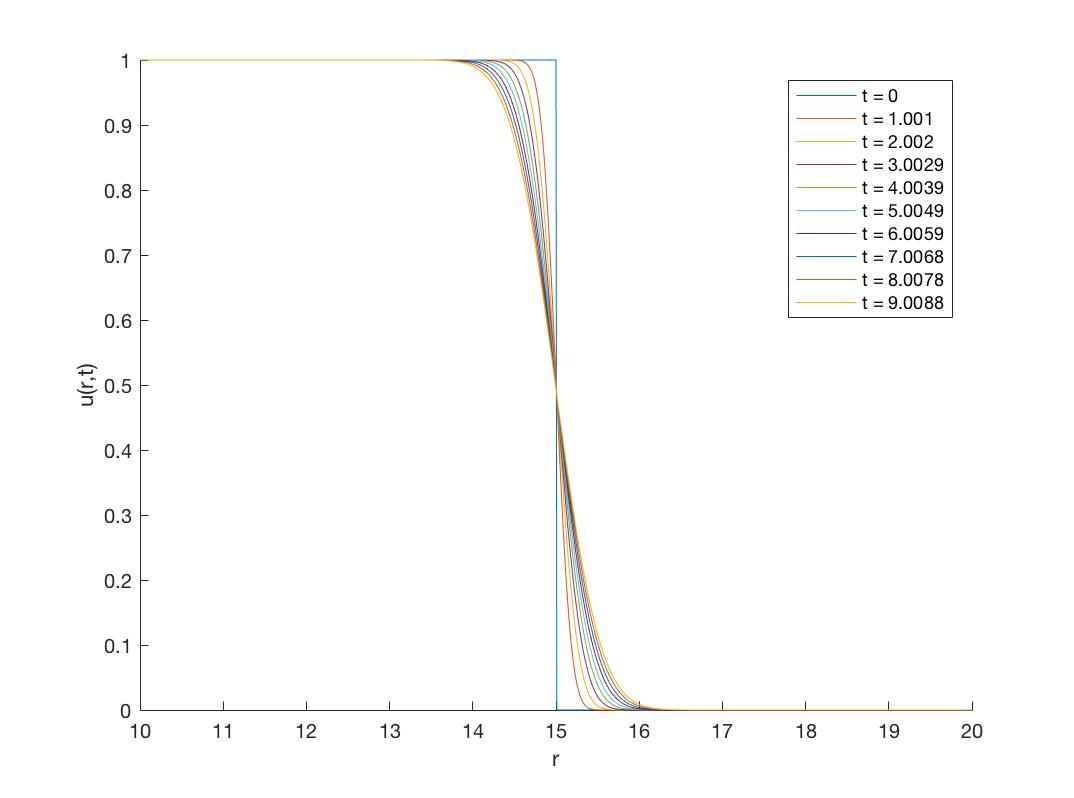
\includegraphics[width = 0.75\textwidth]{fig_q1}
		\caption{ $r$ vs $u(r,t)$ \\ for t $ = 0$ to $10$ with $a=10, b=20$,$Q = 0.01$, $D = 0.01$, $N = 2^{10}$, $Nt = 2^{12}$}
	\end{figure}

	And the contour plot for this initial condition with the specified boundary condition gives 
	
	\begin{figure}[h!]
		\centering
		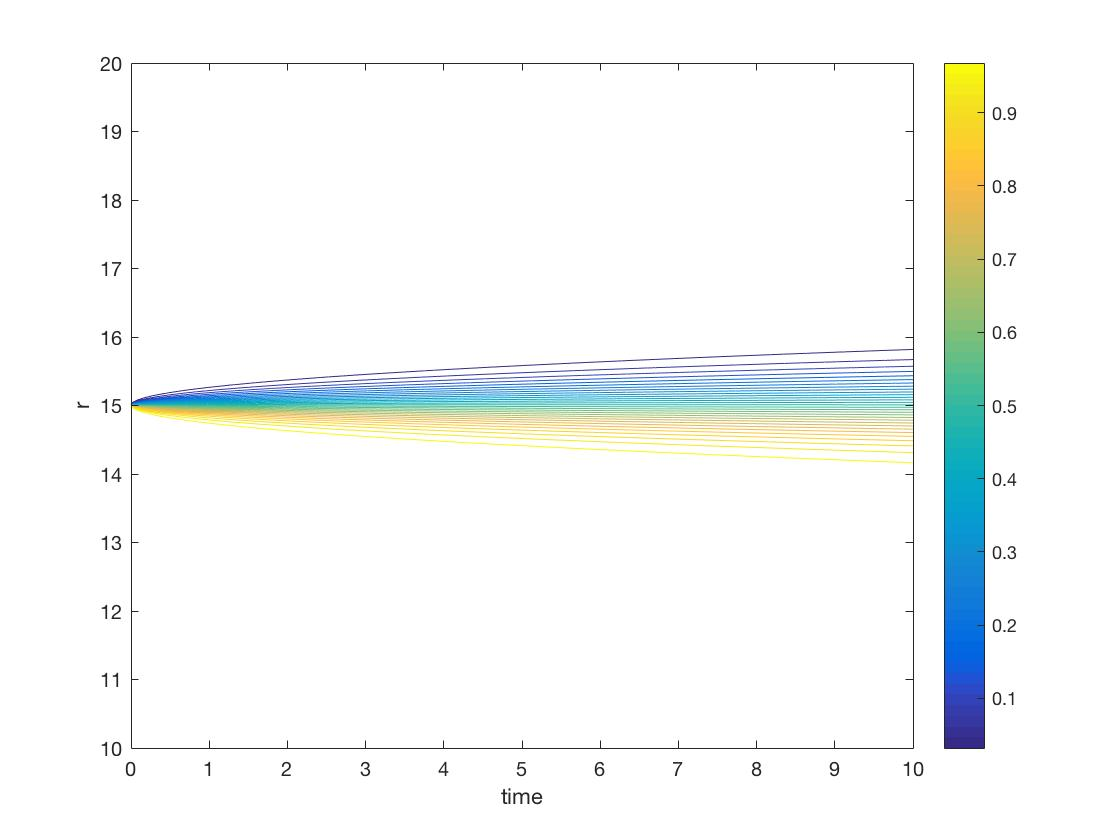
\includegraphics[width = 0.7\textwidth]{fig_q1contour}
		\caption{ Contour plot of $t$ vs $r$ \\ with $a=10, b=20$,$Q = 0.01$, $D = 0.01$, $N = 2^{10}$, $Nt = 2^{12}$}
	\end{figure}
	
	%%%%%%%%%%%%%%%%%%%%%%%%%%%%%%%%%%%%%%%%%%%%%%%%%%%%%%%%%%%
	\newpage
	\item For this section I have chosen the function 
	
	\begin{equation}
		u(r,t) = \frac{b - r}{b - a} + (r-a) (r-b) e^{-t}
	\end{equation}

	that satisfies the boundary conditions specified. Namely $u(a,t) = 1$ and $u(b,t) = 0$. 
	
	The given equation ($\star$) can be rearranged to for $S(r,t)$ to give
	
	\begin{equation}
		\begin{split}
			S(r,t) &= u_t - (\frac{Q}{r} u_r - D (u_rr + \frac{u_r}{r}) \\
		\end{split}
	\end{equation}
	
	For my chosen function the unknown terms are
	
	\begin{equation}
	\begin{split}
		u_t &= - (r-b) (r-a) e^{-t} \\
        u_r &= - \frac{1}{b-a} + ( 2r - a - b ) e^{-t} \\
        u_rr &= 2e^{-t}
    \end{split}
	\end{equation}
	
	which can be combined to explicitly give $S(r,t)$. $u_0(r)$ is
	
	\begin{equation}
		u_0(r) = \frac{b - r}{b - a} + (r-a)(r-b)
	\end{equation}
	
	Furthermore my chosen constant values are
	
	\begin{equation}
		\begin{split}
			a &= 1\\
			b &= 2\\
			D &= 0.01\\
			Q &= 0.01\\
		\end{split}
	\end{equation}
	
	This function can be solved using the code in \texttt{solveq2.m}. 
	
	Now to check whether the error behaves according to $\mathcal{O}(k,h^2)$ I consider the point $(r_0,t_0) = (1.5, 4)$.
	
	Using the code in \texttt{q2error\_k.m} I find that the error does indeed grow linearly with $k$.
	
	\begin{figure}[h!]
		\centering
		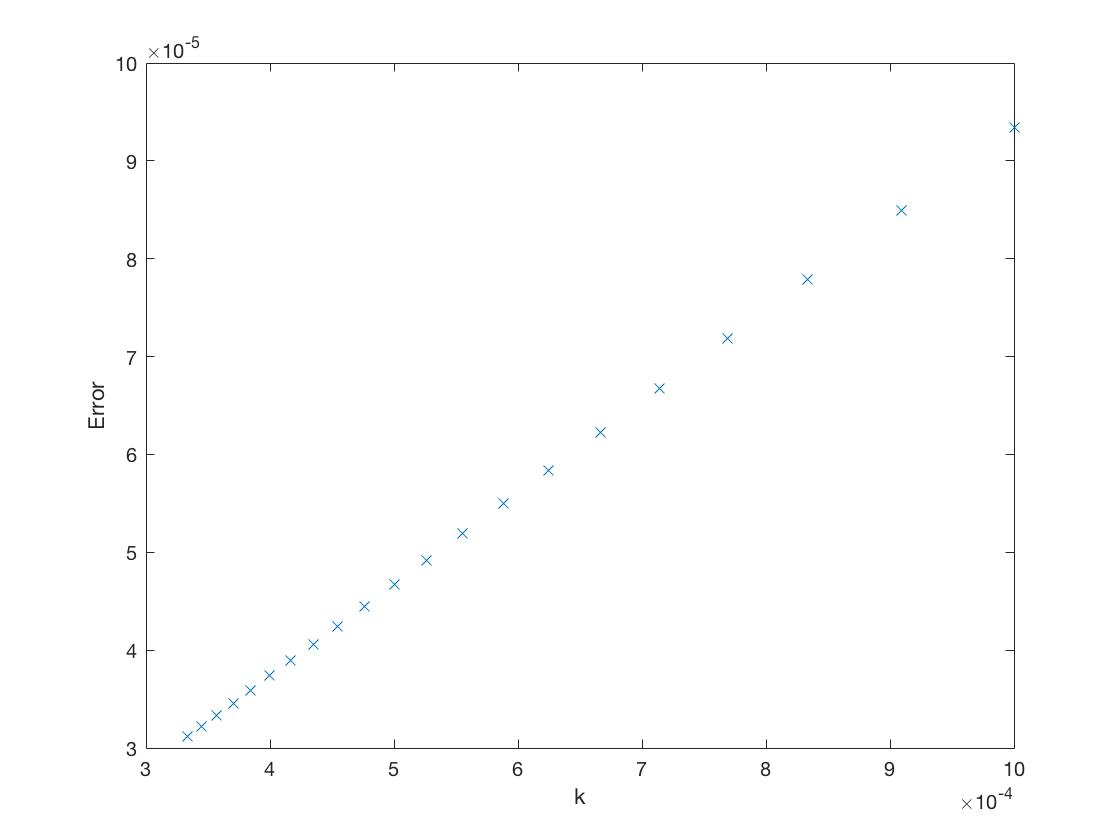
\includegraphics[width = 0.75\textwidth]{fig_q2ek}
		\caption{k vs Error}
	\end{figure}
	
	Using the code in \texttt{q2error\_h.m} I find that the error grows quadratically with $h$.
	
	\begin{figure}[h!]
		\centering
		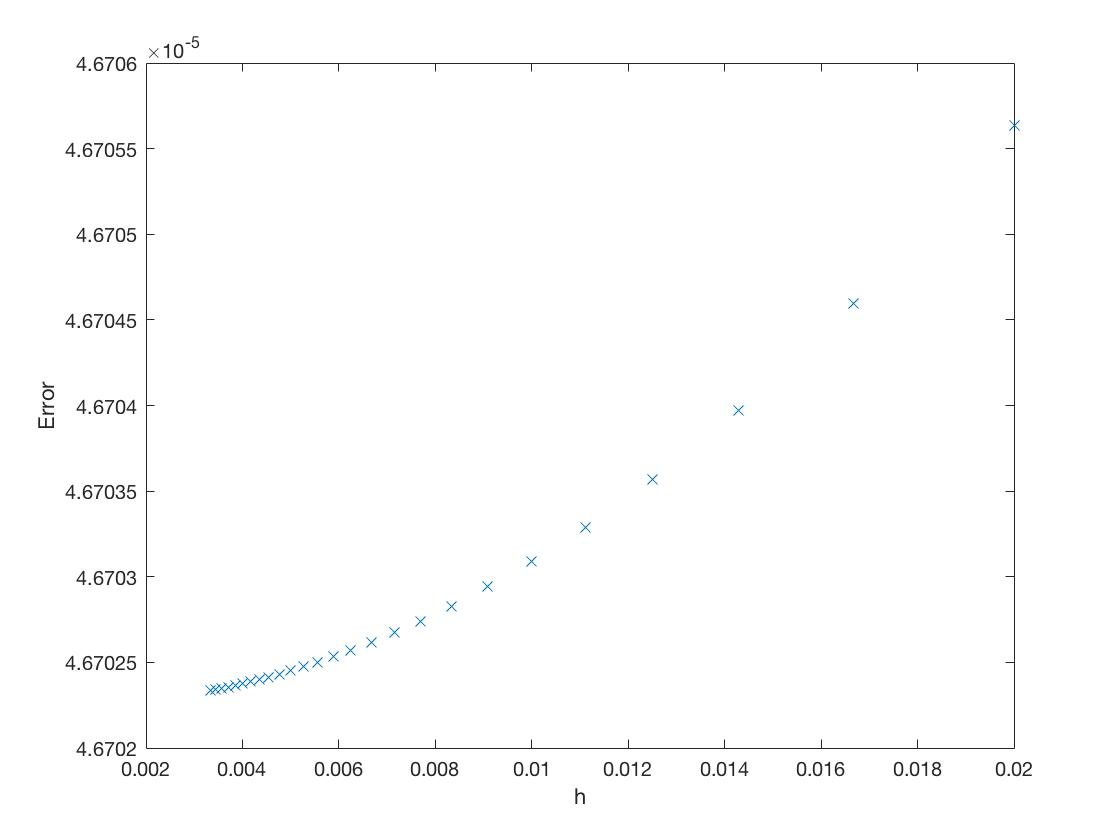
\includegraphics[width = 0.75\textwidth]{fig_q2eh}
		\caption{h vs Error}
	\end{figure}
%%%%%%%%%%%%%%%%%%%%%%%%%%%%%%%%%%%%%%%%%%%%%%%%%%%%%%%%%%%

	\item Since the equation above is similar to the advection equation dealt with in lecture 3-4, the stability analysis can be carried out in the same way as before. 
	
	So 
	
	\begin{equation}
		\boldsymbol{\Phi}(r,t,u,u_r,u_rr) = \frac{Q+D}{r}u_r + Du_{rr} + S(r,t)
	\end{equation}
	
	which gives 
	
	\begin{equation}
		\frac{\partial \boldsymbol{\Phi}}{\partial u_{rr}} = D \quad \text{,} \quad \frac{\partial \boldsymbol{\Phi}}{\partial u_{r}} = \frac{Q+D}{r} \quad \text{and} \quad \frac{\partial \boldsymbol{\Phi}}{\partial u} = 0
	\end{equation}
	
	and so the stability conditions are 
	
	\begin{equation}
		\frac{k}{h^2} \leq \frac{1}{2D} \quad \text{and} \quad \frac{h}{2} \leq D|\frac{a}{D+Q}|
	\end{equation}
	
	The same function as in the previous part has been used to analyse the stability conditions of the code.
	
	Note that $\frac{1}{2D} = 50$ and that $2D|\frac{a}{D+Q}| = 1$. So by changing h and k the upper bounds can be achieved.
	
	Setting $h = 0.01$ gives $k \leq \frac{h^2}{2D} = 0.005$. So for $k = \frac{4}{800} = 0.005$ the code works but for $k = \frac{4}{780} > 0.005$ the solution starts to become unstable. See the code in \texttt{q3.m} for a implemented example.
	
	The second condition is overly cautious and going over it doesn't make the solution unstable.
	
%%%%%%%%%%%%%%%%%%%%%%%%%%%%%%%%%%%%%%%%%%%%%%%%%%%%%%%%%%%

	\item $u_\infty(r)$ is found by iterating in time until the solution converges to some pre-specified tolerance. This is done in the code in \texttt{solveq4.m} where the tolerance is set to $10^{-10}$ although this can be altered very easily. Convergence of the solution is measured by comparing it to the norm of the difference between the solution at each iteration. That is until

	\begin{equation}
		||u^{(j+1)} - u^{(j)}|| < \text{Tolerance}
	\end{equation}
	
	The values chosen for this part of the question are
	
	\begin{equation}
		\begin{split}
			a &= 1\\
			b &= 17\\
			k &= 0.01\\
			h &= 16/512 = 0.03125\\
			D &= 0.01
		\end{split}
	\end{equation}
	
	This gives a ratio of $\frac{b}{a} = 17$. The following plot shows some values of $\frac{Q}{D}$.
	
	\begin{figure}[h!]
		\centering
		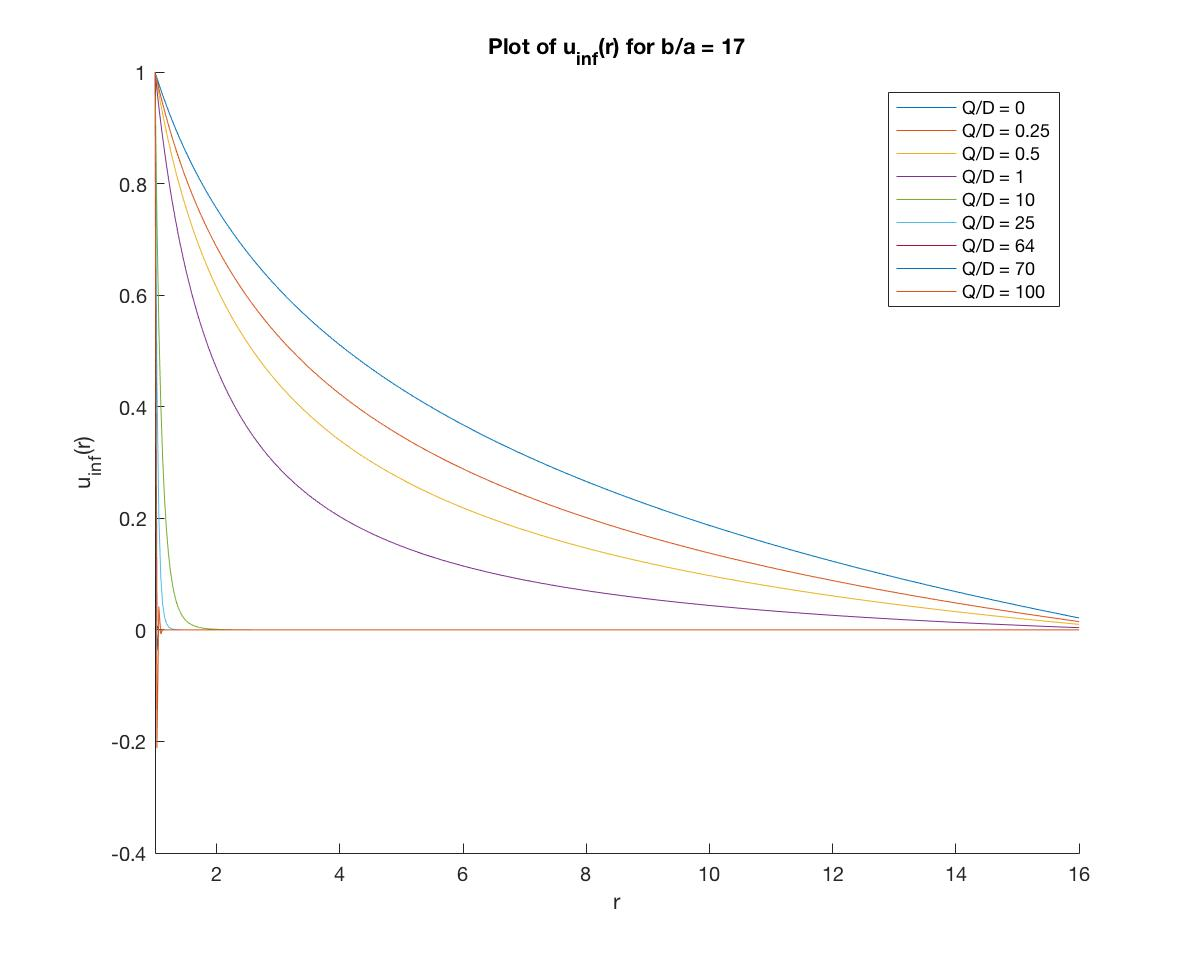
\includegraphics[width = \textwidth]{fig_q4.jpg}
		
		\caption{Various values of $Q/D$ for $u_\infty(r)$ with a tolerance of $10^{-10}$. From \texttt{q4.m}}
	\end{figure}
	
	It can be seen that as $Q/D$ increases the curve gets steeper which is reasonable as the effect of advection is much stronger than that of diffusion meaning the concentration of the drug is directed towards the centre of the annulus. 
	
	As $Q/D$ gets much larger as the slope becomes steeper this method becomes numerically unstable. This is to be expected as one of the stability conditions is $h < 2D|\frac{2a}{Q+D}|$. As $Q/D$ increases this can be estimated as $$ 2D|\frac{2a}{Q+D}| \approx \frac{2Da}{Q} \rightarrow 0$$ and so will eventually be smaller than the chosen value for $h$.
	
	In this case $h = 0.01$ and so the scheme stops working when $\frac{D}{Q} < \frac{h}{2}$, i.e. when $Q/D > 64$. The figure above agrees with this result as the code works for $Q/D = 64$ but becomes unstable for $Q/D = 70$ and $Q/D = 100$.

	Note that the first stability condition is always satisfied here as 
	
	\begin{equation*}
		10 \approx \frac{k}{h^2} < \frac{1}{2D} = 50
	\end{equation*}
	
\end{enumerate}

	Find all the code attached in the zip file along with the submission

\end{document}
